% Options for packages loaded elsewhere
% Options for packages loaded elsewhere
\PassOptionsToPackage{unicode}{hyperref}
\PassOptionsToPackage{hyphens}{url}
\PassOptionsToPackage{dvipsnames,svgnames,x11names}{xcolor}
%
\documentclass[
  sn-basic,
]{sn-jnl}


\usepackage{xcolor}
\usepackage{amsmath,amssymb}
\setcounter{secnumdepth}{5}
\usepackage{iftex}
\ifPDFTeX
  \usepackage[T1]{fontenc}
  \usepackage[utf8]{inputenc}
  \usepackage{textcomp} % provide euro and other symbols
\else % if luatex or xetex
  \usepackage{unicode-math} % this also loads fontspec
  \defaultfontfeatures{Scale=MatchLowercase}
  \defaultfontfeatures[\rmfamily]{Ligatures=TeX,Scale=1}
\fi
\usepackage{lmodern}
\ifPDFTeX\else
  % xetex/luatex font selection
\fi
% Use upquote if available, for straight quotes in verbatim environments
\IfFileExists{upquote.sty}{\usepackage{upquote}}{}
\IfFileExists{microtype.sty}{% use microtype if available
  \usepackage[]{microtype}
  \UseMicrotypeSet[protrusion]{basicmath} % disable protrusion for tt fonts
}{}
\makeatletter
\@ifundefined{KOMAClassName}{% if non-KOMA class
  \IfFileExists{parskip.sty}{%
    \usepackage{parskip}
  }{% else
    \setlength{\parindent}{0pt}
    \setlength{\parskip}{6pt plus 2pt minus 1pt}}
}{% if KOMA class
  \KOMAoptions{parskip=half}}
\makeatother
% Make \paragraph and \subparagraph free-standing
\makeatletter
\ifx\paragraph\undefined\else
  \let\oldparagraph\paragraph
  \renewcommand{\paragraph}{
    \@ifstar
      \xxxParagraphStar
      \xxxParagraphNoStar
  }
  \newcommand{\xxxParagraphStar}[1]{\oldparagraph*{#1}\mbox{}}
  \newcommand{\xxxParagraphNoStar}[1]{\oldparagraph{#1}\mbox{}}
\fi
\ifx\subparagraph\undefined\else
  \let\oldsubparagraph\subparagraph
  \renewcommand{\subparagraph}{
    \@ifstar
      \xxxSubParagraphStar
      \xxxSubParagraphNoStar
  }
  \newcommand{\xxxSubParagraphStar}[1]{\oldsubparagraph*{#1}\mbox{}}
  \newcommand{\xxxSubParagraphNoStar}[1]{\oldsubparagraph{#1}\mbox{}}
\fi
\makeatother


\usepackage{longtable,booktabs,array}
\usepackage{calc} % for calculating minipage widths
% Correct order of tables after \paragraph or \subparagraph
\usepackage{etoolbox}
\makeatletter
\patchcmd\longtable{\par}{\if@noskipsec\mbox{}\fi\par}{}{}
\makeatother
% Allow footnotes in longtable head/foot
\IfFileExists{footnotehyper.sty}{\usepackage{footnotehyper}}{\usepackage{footnote}}
\makesavenoteenv{longtable}
\usepackage{graphicx}
\makeatletter
\newsavebox\pandoc@box
\newcommand*\pandocbounded[1]{% scales image to fit in text height/width
  \sbox\pandoc@box{#1}%
  \Gscale@div\@tempa{\textheight}{\dimexpr\ht\pandoc@box+\dp\pandoc@box\relax}%
  \Gscale@div\@tempb{\linewidth}{\wd\pandoc@box}%
  \ifdim\@tempb\p@<\@tempa\p@\let\@tempa\@tempb\fi% select the smaller of both
  \ifdim\@tempa\p@<\p@\scalebox{\@tempa}{\usebox\pandoc@box}%
  \else\usebox{\pandoc@box}%
  \fi%
}
% Set default figure placement to htbp
\def\fps@figure{htbp}
\makeatother





\setlength{\emergencystretch}{3em} % prevent overfull lines

\providecommand{\tightlist}{%
  \setlength{\itemsep}{0pt}\setlength{\parskip}{0pt}}





%%%% Standard Packages

\usepackage{graphicx}%
\usepackage{multirow}%
\usepackage{amsmath,amssymb,amsfonts}%
\usepackage{amsthm}%
\usepackage{mathrsfs}%
\usepackage[title]{appendix}%
\usepackage{xcolor}%
\usepackage{textcomp}%
\usepackage{manyfoot}%
\usepackage{booktabs}%
\usepackage{algorithm}%
\usepackage{algorithmicx}%
\usepackage{algpseudocode}%
\usepackage{listings}%

%%%%

\raggedbottom
\makeatletter
\@ifpackageloaded{caption}{}{\usepackage{caption}}
\AtBeginDocument{%
\ifdefined\contentsname
  \renewcommand*\contentsname{Table of contents}
\else
  \newcommand\contentsname{Table of contents}
\fi
\ifdefined\listfigurename
  \renewcommand*\listfigurename{List of Figures}
\else
  \newcommand\listfigurename{List of Figures}
\fi
\ifdefined\listtablename
  \renewcommand*\listtablename{List of Tables}
\else
  \newcommand\listtablename{List of Tables}
\fi
\ifdefined\figurename
  \renewcommand*\figurename{Figure}
\else
  \newcommand\figurename{Figure}
\fi
\ifdefined\tablename
  \renewcommand*\tablename{Table}
\else
  \newcommand\tablename{Table}
\fi
}
\@ifpackageloaded{float}{}{\usepackage{float}}
\floatstyle{ruled}
\@ifundefined{c@chapter}{\newfloat{codelisting}{h}{lop}}{\newfloat{codelisting}{h}{lop}[chapter]}
\floatname{codelisting}{Listing}
\newcommand*\listoflistings{\listof{codelisting}{List of Listings}}
\usepackage{amsthm}
\theoremstyle{plain}
\newtheorem{proposition}{Proposition}[section]
\theoremstyle{plain}
\newtheorem{theorem}{Theorem}[section]
\theoremstyle{remark}
\AtBeginDocument{\renewcommand*{\proofname}{Proof}}
\newtheorem*{remark}{Remark}
\newtheorem*{solution}{Solution}
\newtheorem{refremark}{Remark}[section]
\newtheorem{refsolution}{Solution}[section]
\makeatother
\makeatletter
\makeatother
\makeatletter
\@ifpackageloaded{caption}{}{\usepackage{caption}}
\@ifpackageloaded{subcaption}{}{\usepackage{subcaption}}
\makeatother
\usepackage{bookmark}
\IfFileExists{xurl.sty}{\usepackage{xurl}}{} % add URL line breaks if available
\urlstyle{same}
\hypersetup{
  pdftitle={Learning growth mechanisms of tail realistic preferential attachment models from network degree distributions},
  pdfauthor={Thomas William Boughen; Clement Lee; Vianey Palacios Ramirez},
  pdfkeywords={networks, discrete extremes, power law, preferential
attachment},
  colorlinks=true,
  linkcolor={blue},
  filecolor={Maroon},
  citecolor={Blue},
  urlcolor={Blue},
  pdfcreator={LaTeX via pandoc}}


\title[Learning growth mechanisms of tail realistic preferential
attachment models from network degree distributions]{Learning growth
mechanisms of tail realistic preferential attachment models from network
degree distributions}

% author setup
\author[1]{\fnm{Thomas William} \sur{Boughen}}\author[1]{\fnm{Clement} \sur{Lee}}\author[1]{\fnm{Vianey Palacios} \sur{Ramirez}}
% affil setup
\affil[1]{\orgdiv{School of Mathematics, Statistics and
Physics}, \orgname{Newcastle University}}

% abstract 

\abstract{Devising the underlying generating mechanism of a real-life
network is difficult as, more often than not, only its snapshots are
available, but not its full evolution. One candidate for the generating
mechanism is preferential attachment which, in its simplest form,
results in a degree distribution that follows the power law.
Consequently, the growth of real-life networks that roughly display such
power-law behaviour is commonly modelled by preferential attachment.
However, the validity of the power law has been challenged by the
presence of alternatives with comparable performance, as well as the
recent findings that the right tail of the degree distribution is often
lighter than implied by the body, whilst still being heavy. In this
paper, we study a modified version of the model with a flexible
preference function that allows super/sub-linear behaviour whilst also
guaranteeing that the limiting degree distribution has a heavy tail. We
relate the distributions tail index directly to the model parameters,
allowing direct inference of the parameters from the degree distribution
alone.}

% keywords
\keywords{networks,  discrete extremes,  power law,  preferential
attachment}

\begin{document}
\maketitle


\newpage

\section{Introduction}\label{introduction}

Networks have become powerful tools for representing and analysing
complex systems, with uses in a large array of fields. In network
science and statistics, they have been studied by various families of
models, from stochastic block models for detecting communities online
\citep{Latouche11}, to exponential random graph models (ERGMs) for
analysing the global trade network \citep{Setayesh22}, and mechanistic
models for investigating patterns in neural systems \citep{Betzel17}.

Amid the recent rise of interest in networks, there has been a debate on
whether most real networks are scale-free. Claiming a real network is
scale-free is equivalent to saying that its degree distribution follows
a power law, that is the fraction of nodes with degree \(k\) is
proportional to \(k^{-\alpha}\), and therefore has a regularly varying
tail with tail index \(\alpha\). On the side against the claim is
\citet{Broido_2019} who compared the fits of a power law model against
that of several non-scale-free models to nearly a thousand networks,
only to find strong evidence for scale-freeness in four percent and weak
evidence in over half of the networks, thus claiming that scale-free
networks do not make up a majority in real networks. On the other side
of this debate is \citet{Voitalov_2019} who disagrees and claims that
these networks are not nearly as rare and only appear to so as a result
of an unrealistic expectation of a power law without deviations or
noise. Additional evidence of these deviations from a power law is shown
by \citet{Lee24} who demonstrate that a lot of networks are partially
scale-free, in that the body of the degree distribution is often
modelled well by a power law, while the tail is lighter than what is
implied by the body, albeit still regularly varying. Nevertheless, most
studies into the appropriateness of a power law for the degrees of real
networks, the aforementioned references included, have been largely
descriptive in the sense that no information about the growth of the
networks is revealed.

The popularity of using the power law for network degrees can be traced
back to the preferential attachment (PA) model popularised by
\citet{Barabasi99}. In the general model, as new nodes join the network,
an existing node with degree \(k\) gains edges at a rate proportional to
\(b(k)\), where \(b(\cdot)\) is a non-negative preference function.
\citet{Barabasi99} showed that, when \(b(k) = k + 1\), in the limit the
resulting degree distribution is regularly varying with index 2.
Subsequently, if a real network is shown to be scale-free, one can
loosely justify PA as the underlying mechanism of its growth.

The model from \citet{Barabasi99} provided the foundations for various
generalisations --- \citet{krapivsky01} considered
\(b(k) = (k+1)^\alpha\), and showed that the degree distribution is not
regularly varying (and therefore not following the power law) when
\(0<\alpha<1\), and when \(\alpha>1\) a finite number of nodes end up
with all edges after a certain point resulting in a degenerate degree
distribution. \citet{wang2022random} returns to a linear preference
function of the form \(b(k) = k+\varepsilon\) but adds the possibility
for reciprocal edges to be sent, resulting in the joint distribution of
in-degree and out-degree being multivariate regularly varying and having
the property of hidden regular variation. \citet{rudas07} follows in the
footsteps of \citet{krapivsky01}, by considering a PA tree and using
theory from continuous branching processes, derives a limiting degree
distribution in terms of the preference function \(b(\cdot)\).
Nevertheless, research in this area tends to only focus on the
theoretical asymptotic results of network growth models with little
analysis of real networks.

This paper aims to address the gap between the applied and theoretical
works, by asking if a network is assumed to come from a PA model, can we
use the degree distribution alone to directly infer the parameters of
the the preference function and learn about the growth mechanisms?
Moreover, proper consideration is given to the tail of the degree
distribution, because otherwise the effects of the largest degrees,
which correspond to the most influential nodes, deviating from the power
law will be discounted.

As the degrees of networks are discrete values, we will use methods from
discrete extreme value theory, in particular those by \citet{shimura12},
who provided theoretical guarantees for a discrete distribution to be
regularly varying or not. Using these results, we demonstrate how the
tail of the degree distribution is affected by \(b(\cdot)\), and
subsequently propose a class of preference functions that is tail
realistic for real networks. These analytical results enables the
likelihood of the degree distribution to be expressed in terms of the
parameters of \(b(\cdot)\), which in turn allows the underlying
mechanism of the network, assumed to grow according to PA, to be
inferred directly.

The remainder of the paper is as follows: Section~\ref{sec-tail} gives a
detailed description of the PA model alongside the theoretical results
for the survival function of the limiting degree distribution, with a
focus on the tail behaviour in terms of the preference function
\(b(\cdot)\). A class of asymptotically linear preference functions will
be introduced and shown to guarantee regular variation in the degree
distribution while remaining flexible up until a threshold.
Section~\ref{sec-model} utilises the proposed preference function and
illustrates numerically how the tail index of the degree distribution
varies with the model parameters. The simulation study in
Section~\ref{sec-sim} demonstrates that the parameters can be recovered
from fitting the model to only the degree distribution.
Section~\ref{sec-real} fits the model to some real data and provides
posterior estimates for the preference function. Section~\ref{sec-conc}
provides a discussion of this paper and possible avenues for future
work.

\newpage

\section{Tail Behaviour of Preferential Attachment
Model}\label{sec-tail}

The model that we will focus on in this paper is the General
Preferential Attachment (GPA) model in \citet{rudas07} and is defined as
follows:

Starting at time \(t=0\) with an initial network of \(m\) vertices that
each have no edges, at times \(t=1,2,\ldots\) a new vertex is added to
the network bringing with it \(m\) directed edges from the new vertex;
the target for each of these edges are selected from the vertices
already in the network with weights proportional to some non-decreasing
preference function \(b(\cdot)\) of their degree, where
\(b: \mathbb N \mapsto \mathbb R^+\setminus\{0\}\) is such that:

\begin{equation}\phantomsection\label{eq-condb2}{
\sum_{k=0}^\infty\frac{1}{b(k)} = \infty.
}\end{equation}

Special cases of this model include the Barabási-Albert (BA) model when
\(b(k) = k+1\), which in the limit of \(t\rightarrow \infty\) leads to a
power-law degree distribution with tail index 2, and the Uniform
Attachment (UA) model where \(b(k)=c\) leading to a degree distribution
that is not regularly varying.

The survival function of the limiting degree distribution, called the
limiting survival hereafter, under condition \ref{eq-condb2} can be
analytically derived in the case where \(m=1\), which is presented
below.

Consider a continuous time branching process \(\zeta(t)\) driven by a
Markovian pure birth process, with \(\zeta(0)=0\) and birth rates
depending on a non-negative function \(b(\cdot)\):

\[
\Pr(\zeta(t+\text{d}t)=k+1|\zeta(t)=k) = b(k)\text{d}t + o(\text{d}t).
\] Now let \(\Upsilon(t)\) be the tree determined by \(\zeta(t)\) as
follows: \(\Upsilon(t)=\{\emptyset\}\) and \(\Upsilon(t)=G\) where each
existing node \(x\) in \(\Upsilon(t)\) gives birth to a child with rate
\(b(\mathrm{deg}(x, \Upsilon(t))\) independently of the other nodes
where \(\mathrm{deg}(x, \Upsilon(t))\) is the degree of node \(x\) in
the tree \(\Upsilon(t)\) at time \(t\), denote by
\(\Upsilon(t)_{\downarrow x}\) the tree when treating node \(x\) as the
root.

Theorem 1 from \citet{rudas07} states that for the tree \(\Upsilon(t)\)
at time \(t\) and a characteristic function of the tree
\(\varphi(\cdot)\) :

\begin{equation}\phantomsection\label{eq-survlim}{
\lim*{t*\rightarrow\infty}\frac{1}{|\Upsilon(t)|}\sum{x\in\Upsilon(t)}\varphi(\Upsilon(t)\_{\downarrow x}) = \lambda\^\* \int\_0\infty e{-\lambda\^\* t}\mathbb E\left[\varphi(\Upsilon(t))\right]\text{d}t 
}\end{equation}

where \(\lambda^*\) satisfies \(\hat\rho(\lambda^*)=1\) and \(\hat\rho\)
is the Laplace transform of the density of the point process associated
with the pure birth process that corresponds to the growth of an
individual node, that is
\(\hat\rho(\lambda) \coloneq \int_0^\infty e^{-\lambda t}\rho(t)\mathrm{d}t\).

The limiting survival can be viewed as the limit of the empirical
proportion of vertices with degree over a threshold \(k\in\mathbb N\),
that is:

\[
\bar F(k) = \lim_{t\rightarrow\infty}\frac{\sum_{x\in\Upsilon(t)}\mathbb I\left\{\text{deg}(x,\Upsilon(t)_{\downarrow x})>k\right\}}{\sum_{x\in\Upsilon(t)} 1}
\] which can also be written using Equation~\ref{eq-survlim} as:

\begin{equation}\phantomsection\label{eq-surv-origin}{
\bar F(k) = \frac{\int_0^\infty e^{-\lambda^* t}\mathbb E\left[\mathbb I\left\{\text{deg}(x,\Upsilon(t))>k\right\}\right]\text{d}t}{\int_0^\infty e^{-\lambda^* t}\text{d}t} = \prod_{i=0}^k\frac{b(i)}{\lambda^* + b(i)}.
}\end{equation}

Therefore, the corresponding probability mass function of the degree
distribution \(f(k) = \bar F(k-1) - \bar F(k)\) is

\begin{equation}\phantomsection\label{eq-pmf-origin}{
f(k) = \frac{\lambda^*}{\lambda^* + b(k)}\prod_{i=0}^{k-1}\frac{b(i)}{\lambda^*+b(i)}.
}\end{equation}

We are interested in how the tail behaviour of the discrete limiting
degree distribution is affected by the preference function \(b\). In
order to study this, we use the quantity \(\Omega(F, k)\) as stated in
\citet{shimura12} and is repeated below:

For a discrete distribution \(F\) with survival function \(\bar F\) and
\(k\in\mathbb Z^+\) let

\[
\Omega(F,k) = \left(\log\displaystyle\frac{\bar F (k+1)}{\bar F (k+2)}\right)^{-1} - \left(\log\displaystyle\frac{\bar F (k)}{\bar F (k+1)}\right)^{-1}.
\]

The following proposition gives the limiting behaviour of
\(\Omega(F,k)\) when \$F\$ is a limiting degree distribution resulting
from the GPA model with preference function \(b(\cdot)\).

\begin{proposition}[]\protect\hypertarget{prp-omega}{}\label{prp-omega}

If \(\bar F(k) = \prod_{i=0}^k\frac{b(i)}{\lambda^* + b(i)}\) and
\(b(k) \rightarrow \infty\) as \(k\rightarrow \infty\), then \[
\lim_{k\rightarrow\infty}\Omega(F,k) = \lim_{k\rightarrow\infty}\frac{b(k+1)-b(k)}{\lambda^*}.
\]

\end{proposition}

See Appendix \ref{sec-proofs} for the details of the proof.

\citet{shimura12} states that if
\(\lim_{k\rightarrow\infty} \Omega(F,k) = 1/\alpha\) (\(\alpha>0\)),
then \(F\) is regularly varying with \(\bar F(k) \sim k^{-\alpha}\). On
the other hand, if \(\lim_{k\rightarrow\infty} \Omega(F,k) = 0\) then we
will refer to the distribution as light-tailed.

Proposition~\ref{prp-omega} aligns with the result from
\citet{krapivsky01} demonstrating that a sub-linear preference function
will lead to a light-tailed distribution, as
\(\lim_{k\rightarrow\infty} b(k+1)-b(k) = 0\) if \(b(k)=k^\alpha\) where
\(\alpha < 1\). Proposition~\ref{prp-omega} also aligns with the fact
that BA model produces a regularly varying degree distribution, with
tail index 2, by considering the preference function
\(b(k) = k + \varepsilon\), as
\(\lim_{k\rightarrow\infty}b(k+1)-b(k)=1\), leaving the tail index to be
\(1/\lambda^*\) which using \(\hat\rho\) can be found to be \(1/2\). So,
in order for the degree distribution to be regularly varying we need
that the limit \(\lim_{k\rightarrow\infty} b(k+1)-b(k)\) exists and is
positive. The following proposition determines the class of functions
that will result in regular varying degree distributions.

\begin{proposition}[]\protect\hypertarget{prp-omega2}{}\label{prp-omega2}

The limiting survival of a GPA model is regularly varying if and only if
the preference function is \emph{eventually} of the form:

\begin{align*}
b(k) &= \beta k + r(k),\\
&\text{and}\\
r(k+1)-r(k)&\rightarrow 0,
\end{align*}

and if the preference function is of this form then the tail index is
exactly \(\lambda^*/\beta\) where \(\hat\rho(\lambda\^\*) = 1\).

\emph{Proof}

Letting \(b(k) = \beta k  + o(k)\) and using Proposition~\ref{prp-omega}
we have that:

\[
\lim_{k\rightarrow\infty}\Omega(F,k) = \lim_{k\rightarrow\infty}\frac{b(k+1)-b(k)}{\lambda^*} = \lim_{k\rightarrow\infty} \frac{\beta + o(k+1) - o(k)}{\lambda^*} = \frac{\beta}{\lambda^*},
\]

and thus the tail index of the limiting survival must be
\(\lambda^*/\beta\).

\hfill\break
If we now assume that the limiting survival is regularly varying with
tail index \(\delta\), we must have that:

\[
\lim_{k\rightarrow\infty}\Omega(F,k) = \delta
\]

and again by Proposition~\ref{prp-omega}

\[
\lim_{k\rightarrow\infty}\frac{b(k+1)-b(k)}{\lambda^*} = \delta
\]

Letting \(b_k=b(k)\) and \(a_k = k\) we can use the Stolz-Cesàro theorem
(Theorem~\ref{thm-stolz}) to obtain:

\[
\lim_{k\rightarrow\infty}\frac{b_{k+1}-b_k}{a_{k+1}-a_k} = \delta \implies \lim_{k\rightarrow\infty}\frac{b_k}{a_k} = \delta
\]

and so

\[
\lim_{k\rightarrow\infty}\frac{b(k)}{k} = \delta
\]

which \(b(k) = \beta k + o(k)\) fulfills.\(\square\)

\end{proposition}

Using this result we can understand how the preference function is
directly connected with the tail behaviour of the degree distribution.
Specifically, regular variation is achieved if and only if \(b(k)\) is
asymptotically linear with \(k\). We use this result to create a
preference function that guarantees regular variation in the tail of the
degree distribution, aligning with analysis of real networks, whilst
allowing for the tail to deviate from the shape implied by the body.
This gives the model the capability to produce realistic behaviour in
the degrees like what was in \citet{Lee24} by using a piecewise function
inspired by the observed deviation from the power law after a certain
threshold:

\begin{equation}\phantomsection\label{eq-pref}{
b(k) = \begin{cases}
k^\alpha + \varepsilon,&k<k_0,\\
k_0^\alpha + \varepsilon + \beta(k-k_0), &k\ge k_0
\end{cases}
}\end{equation} for \(\alpha,\beta, \varepsilon>0\) and
\(k_0\in\mathbb N\).

Using Proposition~\ref{prp-omega}, we can show that
\(\lim_{n\rightarrow\infty}\Omega(F,k)=\lambda^{*}/\beta\), meaning the
degree distribution obtained using this preference function is regularly
varying with tail index \(\lambda^*/\beta\).

\newpage

\section{A PA Model with Flexible Regular Variation}\label{sec-model}

In the previous section, we found that using an asymptotically linear
preference function allows for the inclusion of sub/super-linear
behaviour below the threshold, while simultaneously guaranteeing regular
variation of the degrees. In this section, we demonstrate the
flexibility of the preference function in Equation~\ref{eq-pref}, with
regard to the tail behaviour of the limiting degree distribution. Using
Equation~\ref{eq-surv-origin}, the limiting survival is

\begin{equation}\phantomsection\label{eq-polysurv}{
\bar F(k) = \begin{cases}
\prod_{i=0}^{k}\frac{i^\alpha + \varepsilon}{\lambda^*+i^\alpha + \varepsilon},&k<k_0,\\
\left(\prod_{i=0}^{k_0-1}\frac{i^\alpha + \varepsilon}{\lambda^*+i^\alpha + \varepsilon}\right)\frac{\Gamma(\lambda^*+k_0^\alpha + \varepsilon)/\beta)}{\Gamma\left((k_0^\alpha + \varepsilon)/\beta\right)} \frac{\Gamma\left(k-k_0 + 1 +\frac{k_0^\alpha + \varepsilon}{\beta}\right)}{\Gamma\left(k-k_0 + 1 +\frac{\lambda^* +k_0^\alpha + \varepsilon}{\beta}\right)},&k\ge k_0,
\end{cases}
}\end{equation}

with \(\lambda^*\) satisfying \(\hat \rho(\lambda^*)=1\) where

\begin{equation}\phantomsection\label{eq-rho}{
\hat\rho(\lambda) = \sum_{n=0}^{k_0}\prod_{i=0}^{n-1}\frac{i^\alpha + \varepsilon}{\lambda+i^\alpha + \varepsilon} + \left(\frac{k_0^\alpha + \varepsilon}{\lambda-\beta}\right)\prod_{i=0}^{k_0-1}\frac{i^\alpha + \varepsilon}{\lambda + i^\alpha + \varepsilon} 
}\end{equation}

which has to be solved numerically for most parameter choices. Also,
note that \(\lambda>\beta\).

For some parameter combinations, the limiting survival \(\bar F(k)\) is
shown on log-log scale in Figure~\ref{fig-polylinsurv}:

\begin{figure}

\centering{

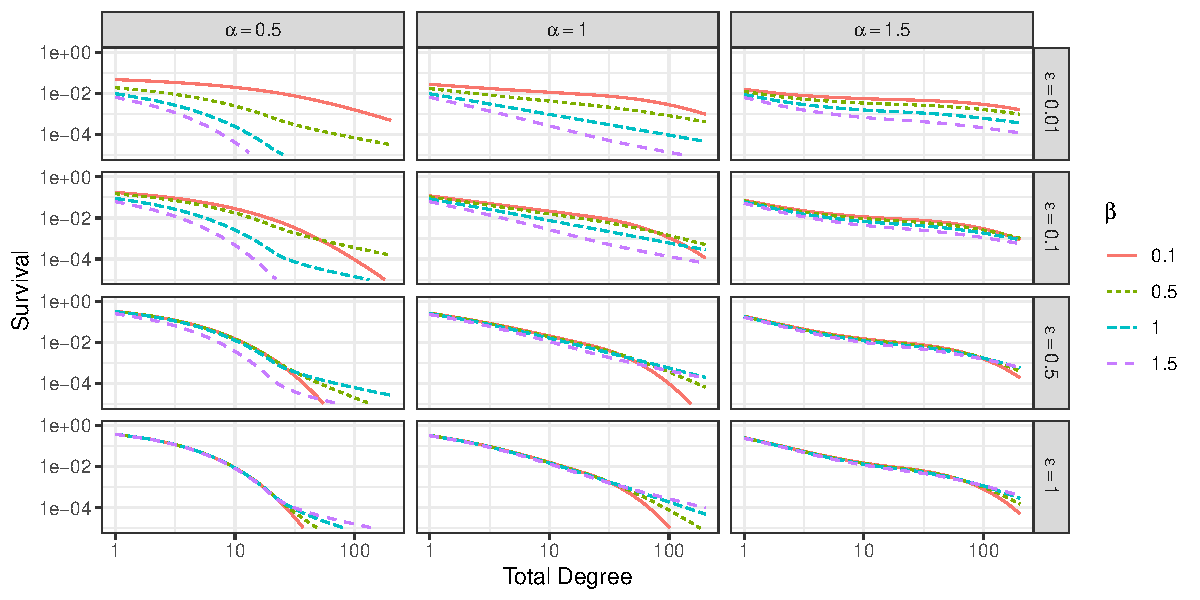
\includegraphics[width=0.8\linewidth,height=\textheight,keepaspectratio]{paper_files/figure-pdf/fig-polylinsurv-1.pdf}

}

\caption{\label{fig-polylinsurv}The limiting survival, according to
various combinations of \((\alpha, \beta, \varepsilon)\) and \(k_0=20\)
of the proposed PA model.}

\end{figure}%

Figure~\ref{fig-polylinsurv} demonstrates that this model can capture a
range of tail behaviour, including a large range of possible tail
indices ranging from 0.035 (\(\alpha=1.5, \beta=0.1, \varepsilon=1\)) to
0.999 (\(\alpha=0.5, \beta=1.5, \varepsilon=0.01\)).

The analytic form of the survival function in (\ref{eq-polysurv}),
offers a natural connection to the discrete version of the generalised
Pareto (GP) distribution , providing a link to a well established
component of discrete extremes in the literature. Specifically, it is
connected to the Integer GP (IGP) distribution seen in
\citet{Rohrbeck_2018} with conditional survival: \[
\Pr(X> x|X> v) = \left(\frac{\xi(x-v)}{\sigma} + 1\right)^{-1/\xi},\qquad x=v+1,v+2,\ldots
\] for \(v\in\mathbb Z^+, \sigma>0,\xi\in \mathbb R\), denoted as
\(X|X>u \sim  \mathrm {IGP}(\xi, \sigma, u)\) where \(\xi\) is the shape
parameter and reciprocal of the tail index.

By Equation~\ref{eq-polysurv} and using Stirling's approximation:

\begin{align*}
\bar F(k|k\ge k_0) &= \frac{\Gamma\left(\frac{\lambda^* + k_0^\alpha + \varepsilon}{\beta}\right)}{\Gamma\left(\frac{k_0^\alpha + \varepsilon}{\beta}\right)}\times\frac{\Gamma\left(k-k_0  +1 + \frac{k_0^\alpha + \varepsilon}{\beta}\right)}{\Gamma\left(k-k_0  +1 + \frac{\lambda^*+ k_0^\alpha + \varepsilon}{\beta}\right)}\\
&\approx\left(\frac{k_0^\alpha+\varepsilon}{\beta}\right)^{\lambda^*/\beta}\left(k-k_0+1+\frac{k_0^\alpha + \varepsilon}{\beta}\right)^{-\lambda^*/\beta}\\
&=\left(\frac{k_0^\alpha+\varepsilon}{k_0^\alpha+\varepsilon + \beta}\right)^{\lambda^*/\beta}\left(\frac{\beta(k-k_0)}{\beta + k_0^\alpha+\varepsilon} + 1\right)^{-\lambda^*/\beta}\\
&=\left(\frac{\beta(k+1-k_0)}{k_0^{\alpha}+\varepsilon} + 1\right)^{-\lambda^{*}/\beta}.
\end{align*}

Therefore, \begin{equation}\phantomsection\label{eq-igp-est}{
\bar F(k) 
\begin{cases}
=\prod_{i=0}^{k}\frac{i^\alpha + \varepsilon}{\lambda^*+i^\alpha + \varepsilon},&k<k_0,\\
\approx \left(\prod_{i=0}^{k_0-1}\frac{i^\alpha + \varepsilon}{\lambda^*+i^\alpha + \varepsilon}\right) \left(\frac{\beta(k+1-k_0)}{k_0^{\alpha}+\varepsilon} + 1\right)^{-\lambda^*/\beta},&k\ge k_0,
\end{cases}
}\end{equation} meaning that for \(k\ge k_0\) the limiting degree
distribution (for large \(k_0^\alpha\)) is approximated by the
\(\text{IGP}\left(\frac{\beta}{\lambda^*}, \frac{k_0^\alpha + \varepsilon}{\lambda^*},k_0-1\right)\)
distribution.

To assess how close of an approximation this is, the theoretical
conditional survival Equation~\ref{eq-polysurv} are shown in
Figure~\ref{fig-approx_surv} in colour and their IGP approximations
Equation~\ref{eq-igp-est} are shown in grey. The approximation holds up
fairly well even for large degrees and more so when \(\alpha\) is
larger.

\begin{figure}

\centering{

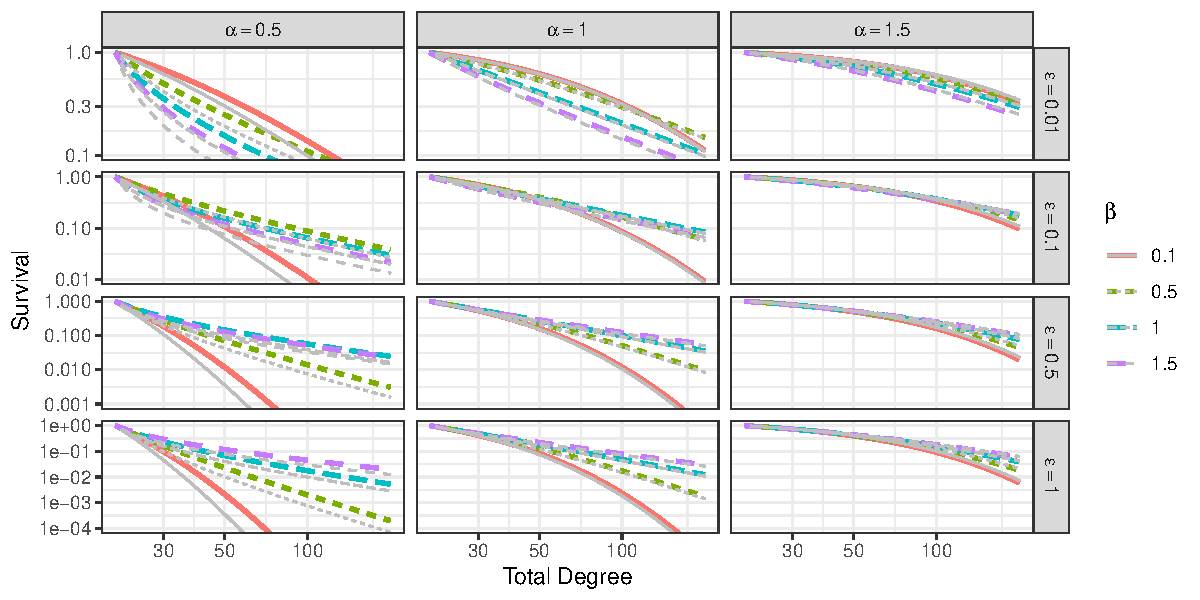
\includegraphics[width=0.8\linewidth,height=\textheight,keepaspectratio]{paper_files/figure-pdf/fig-approx_surv-1.pdf}

}

\caption{\label{fig-approx_surv}Theoretical conditional survivals (grey)
of the proposed model alongside their IGP approximations (coloured).}

\end{figure}%

In agreement with Proposition~\ref{prp-omega2}, \(\beta>0\) ensures that
the shape parameter of the IGP distribution is positive and thus the
distribution is regularly varying. Additionally the shape parameter
\(\xi\) is shown in Figure~\ref{fig-polyheat} for various parameter
choices. The darker and lighter regions on the heat maps correspond to a
heavier and a lighter tail, respectively, and the red dashed line shows
combinations of \(\alpha\) and \(\beta\) that produce a limiting degree
distribution with the same tail index as the BA model.

Through the connection implied by Equation~\ref{eq-igp-est}, fitting the
proposed model is almost equivalent to fitting the IGP distribution to
the degrees and estimating its parameters. However, instead of only
describing the shape of the degree distribution, we would also gain
estimates for the shape of the preference function, thus gaining a
direct understanding the mechanisms underlying the growth of the
network.

\begin{figure}

\centering{

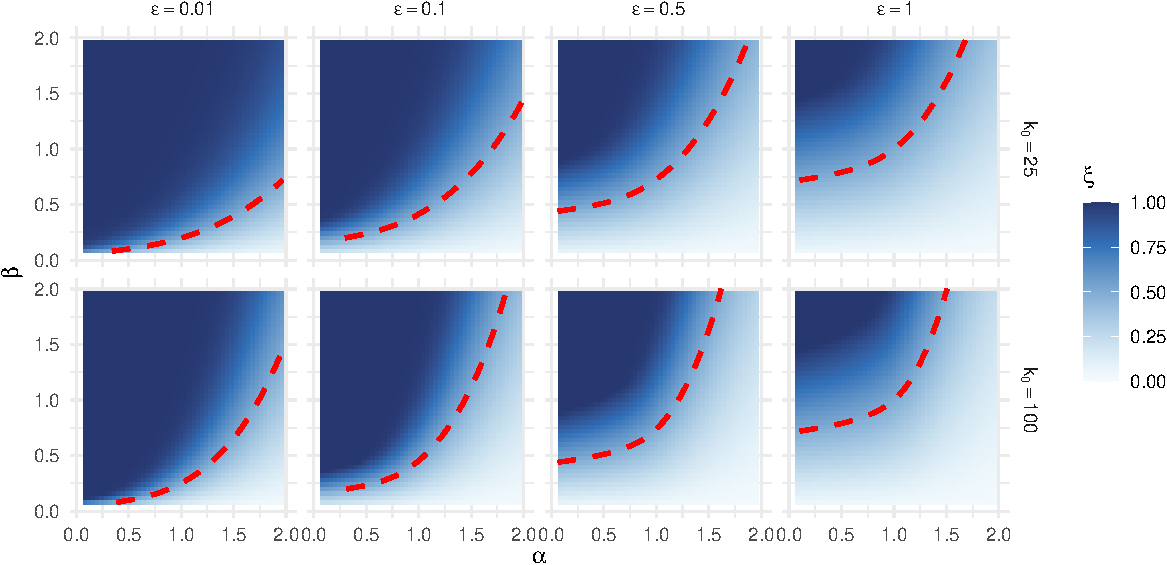
\includegraphics[width=0.8\linewidth,height=\textheight,keepaspectratio]{paper_files/figure-pdf/fig-polyheat-1.pdf}

}

\caption{\label{fig-polyheat}Heat maps of \(\xi\) for various
combinations of the parameters of the proposed model.}

\end{figure}%

\newpage

To perform inference of the model parameters, we consider a network with
degree count vector \(\pmb n = (n_0, n_1, \ldots, n_M)\), where \(M\) is
the maximum degree. Using Equation~\ref{eq-pmf-origin}, the likelihood
is:

\begin{align*}
L(\pmb n | \pmb \theta,l) = &\left(\frac{\lambda^*}{\lambda^*+\varepsilon}\right)^{n_0}\left(\prod_{j=l}^{k_0-1}\frac{j^\alpha +\varepsilon}{\lambda^* + j^\alpha +\varepsilon}\right)^{\left(\sum_{i\ge k_0}n_{i}\right)} \\ &\times \prod_{l \le i<k_0}\left(\frac{\lambda^*}{\lambda^* +i^\alpha + \varepsilon } \prod_{j=l}^{k_0-1}\frac{j^\alpha + \varepsilon}{\lambda^* + j^\alpha + \varepsilon}\right)^{n_i}\\ &\times \prod_{i\ge k_0}\left(\frac{\text{B}(i-k_0 + (k_0^\alpha + \varepsilon)/\beta,1+\lambda^*/\beta)}{\text{B}((k_0^\alpha + \varepsilon)/\beta,\lambda^*/\beta)}\right)^{n_i}
\end{align*}\label{eq-lh}

where \(\text{B}(\cdot,\cdot)\) is the the beta function,
\(\pmb \theta = (\alpha, \varepsilon, k_0,\beta)\), and \(l\ge0\) is a
quantity that allows truncating the data such that the minimum degree is
\(l\). This will allow the model to be fitted whilst ignoring the
influence of the lower degrees (those less than \(l\)) as the model does
not capture the behaviour well at the lower degrees, since
\citet{rudas07} only provides results for the case of a preferential
attachment tree.

\section{Applications}\label{applications}

\subsection{Simulated Data}\label{sec-sim}

This subsection aims to show that the parameters of the model (and
therefore the preference function) in Section~\ref{sec-model} can be
recovered from simulating a network from the model, and fitting it to
the observed degree distribution, using the likelihood in \eqref{eq-lh}.

The procedure for recovering the parameters begins with simulating a
network from the model with \(N=100,000\) vertices and \(m=1\) given
some set of parameters
\(\pmb\theta = (\alpha, \beta, \varepsilon, k_0)\), obtaining the degree
counts and using the likelihood from the previous section alongside the
priors:

\begin{align*}
\alpha&\sim \text{Gamma}(1,0.01),\\
\beta &\sim  \text{Gamma}(1,0.01),\\
k_0 &\sim \text{U}(1,10,000),\\
\varepsilon &\sim \text{Gamma(1,0.01)},
\end{align*}

where Gamma(\(a\), \(b\)) is the gamma distribution with shape \(a\) and
rate \(b\), and U(\(a\), \(b\)) is uniform distribution with lower and
upper bounds \(a\) and \(b\), to obtain a posterior distribution, up to
the proportionality constant. Posterior samples can then be obtained by
an adaptive Metropolis-Hastings Markov chain Monte Carlo (MCMC)
algorithm. For these simulated networks \(l=0\).

\begin{figure}

\centering{

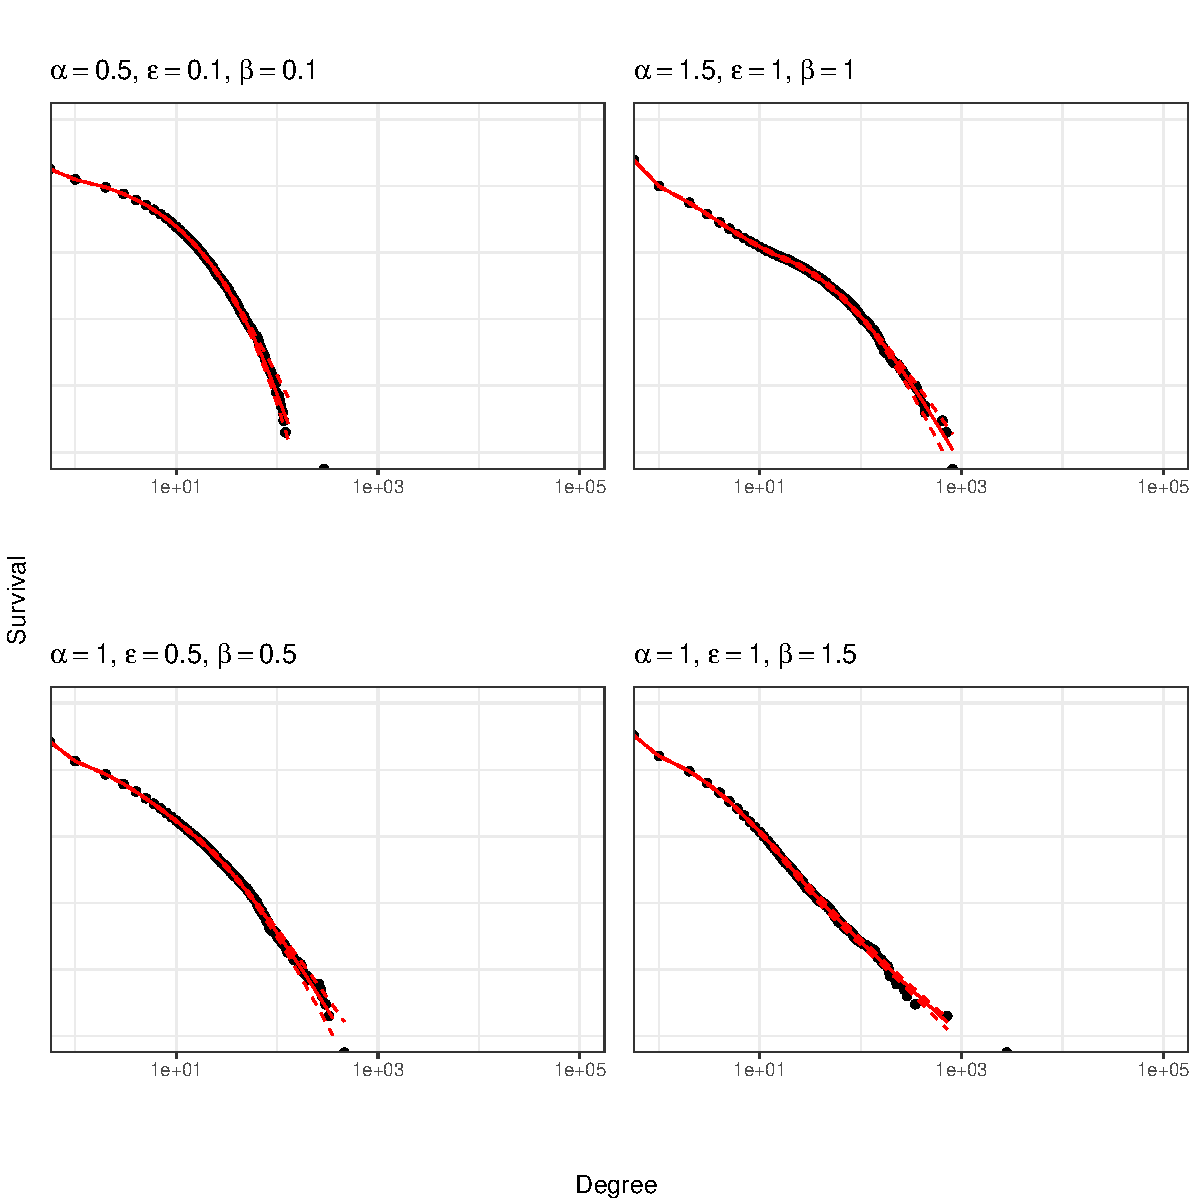
\includegraphics[width=0.8\linewidth,height=\textheight,keepaspectratio]{paper_files/figure-pdf/fig-rec1-1.pdf}

}

\caption{\label{fig-rec1}Empirical (black dots) and fitted (red line)
survival functions for data simulated from the proposed model with
various combinations of \((\alpha,\beta,\epsilon)\) and \(k_0=20\). The
95\% credible (dashed lines) are included but too narrow to be seen
clearly.}

\end{figure}%

\begin{figure}

\centering{

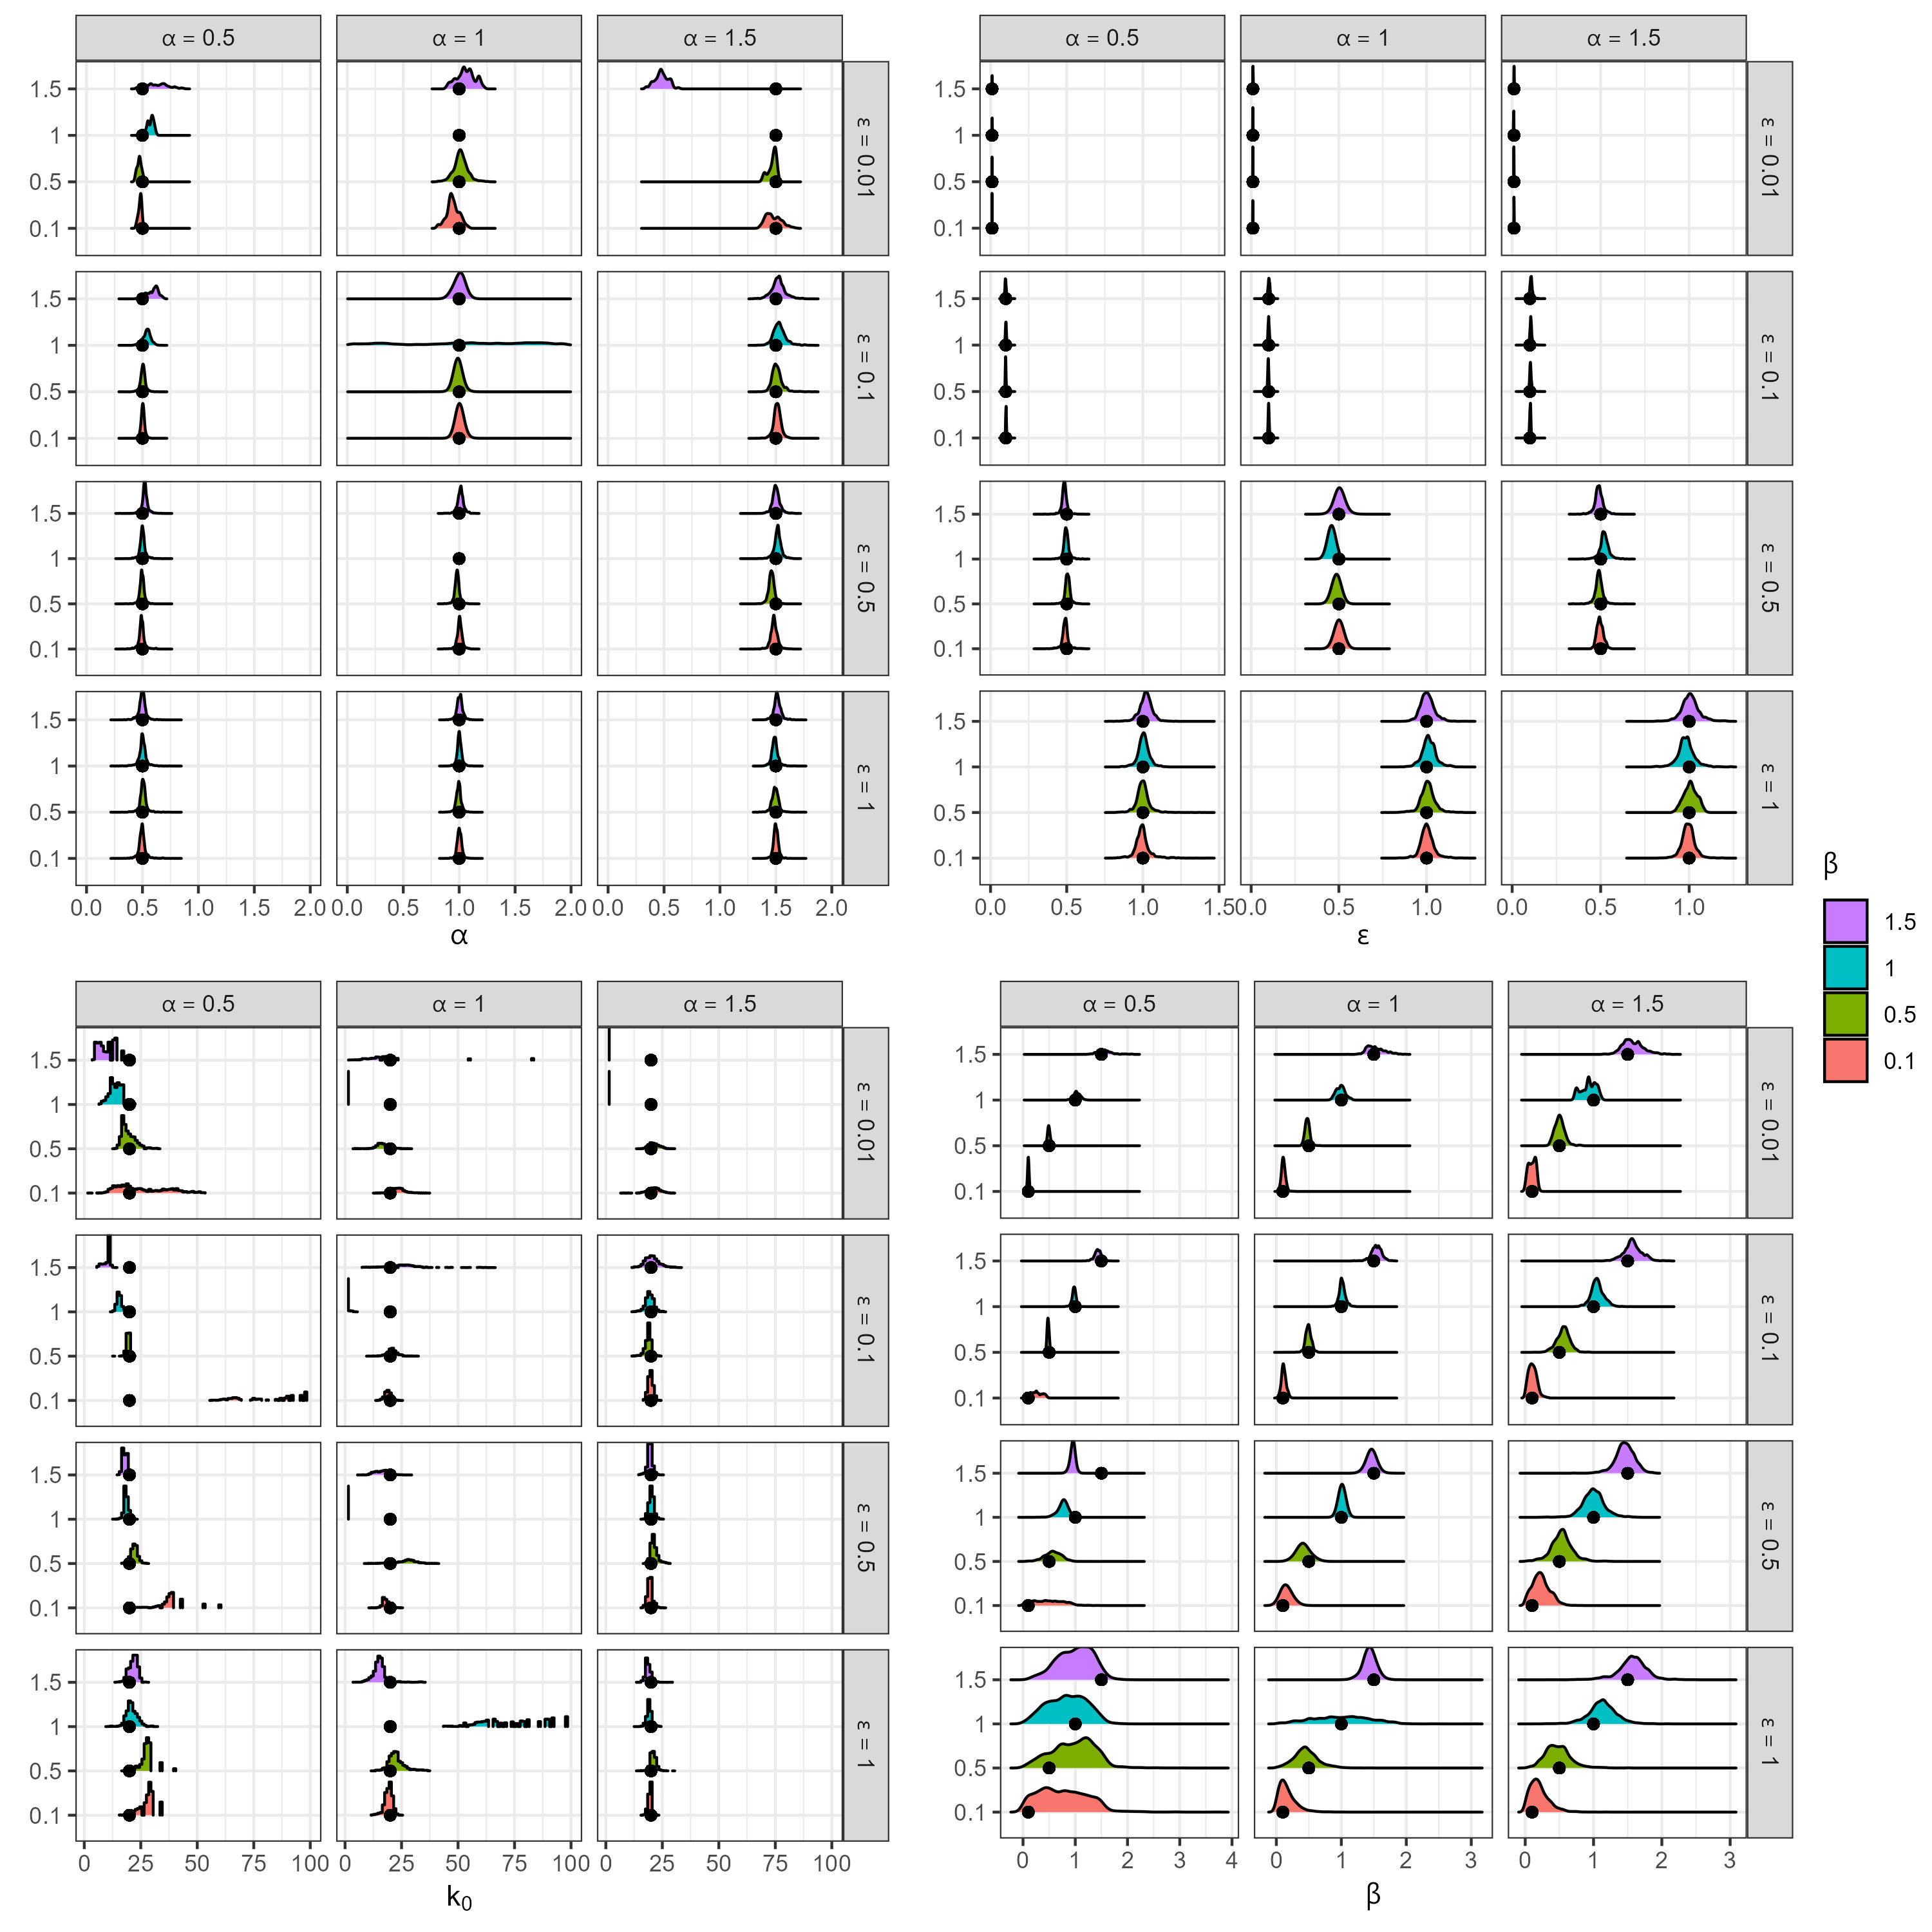
\includegraphics[width=1\linewidth,height=\textheight,keepaspectratio]{images/mcmc_plot.jpg}

}

\caption{\label{fig-rec2}: Posterior densities of parameters for data
simulated from the proposed model with various combinations of
(\(\alpha\),\(\beta\),\(\varepsilon\)) and \(k_0=20\). True parameter
values shown with black dots.}

\end{figure}%

Figures \ref{fig-rec1} and \ref{fig-rec2} demonstrate the usefulness of
the model, as we can recover the model parameters well from only the
final degree distribution of the simulated network. This indicates that
the method may also be applied to real networks, with the assumption
that they evolved according to the GPA scheme.

\subsection{Real Data}\label{sec-real}

In this subsection, we fit the proposed model to the degree
distributions of various real networks and learn about the mechanics of
their growth. While we also compare the fit to that of the mixture
distribution by \citet{Lee24} we note that the proposed method has the
additional benefit of learning directly about the growth of a network
from the inference results. The data consists of 12 networks sourced
from \href{konect.cc}{KONECT} and the
\href{https://networkrepository.com}{Network Data Repository}\citep{nr}:

\begin{itemize}
\tightlist
\item
  \texttt{as-caida20071105}: network of autonomous systems of the
  Internet connected with each other from the CAIDA project
\item
  \texttt{dimacs10-astro-ph} : co-authorship network from the
  ``astrophysics'' section (astro-ph) of arXiv
\item
  \texttt{ego-twitter}: network of twitter followers
\item
  \texttt{facebook-wosn-wall}: subset of network of Facebook wall posts
\item
  \texttt{maayan-faa}: USA FAA (Federal Aviation Administration)
  preferred routes as recommended by the NFDC (National Flight Data
  Center)
\item
  \texttt{maayan-Stelzl}: network representing interacting pairs of
  proteins in humans
\item
  \texttt{moreno-blogs-blogs}: network of URLs found on the first pages
  of individual blogs
\item
  \texttt{opsahl−openflights}: network containing flights between
  airports of the world.
\item
  \texttt{pajek-erdos}: co-authorship network around Paul Erdős
\item
  \texttt{reactome}: network of protein--protein interactions in humans
\item
  \texttt{sx-mathoverflow}: interactions from the StackExchange site
  \href{https://mathoverflow.net/}{MathOverflow}
\item
  \texttt{topology}: network of connections between autonomous systems
  of the Internet
\end{itemize}

\begin{figure}

\centering{

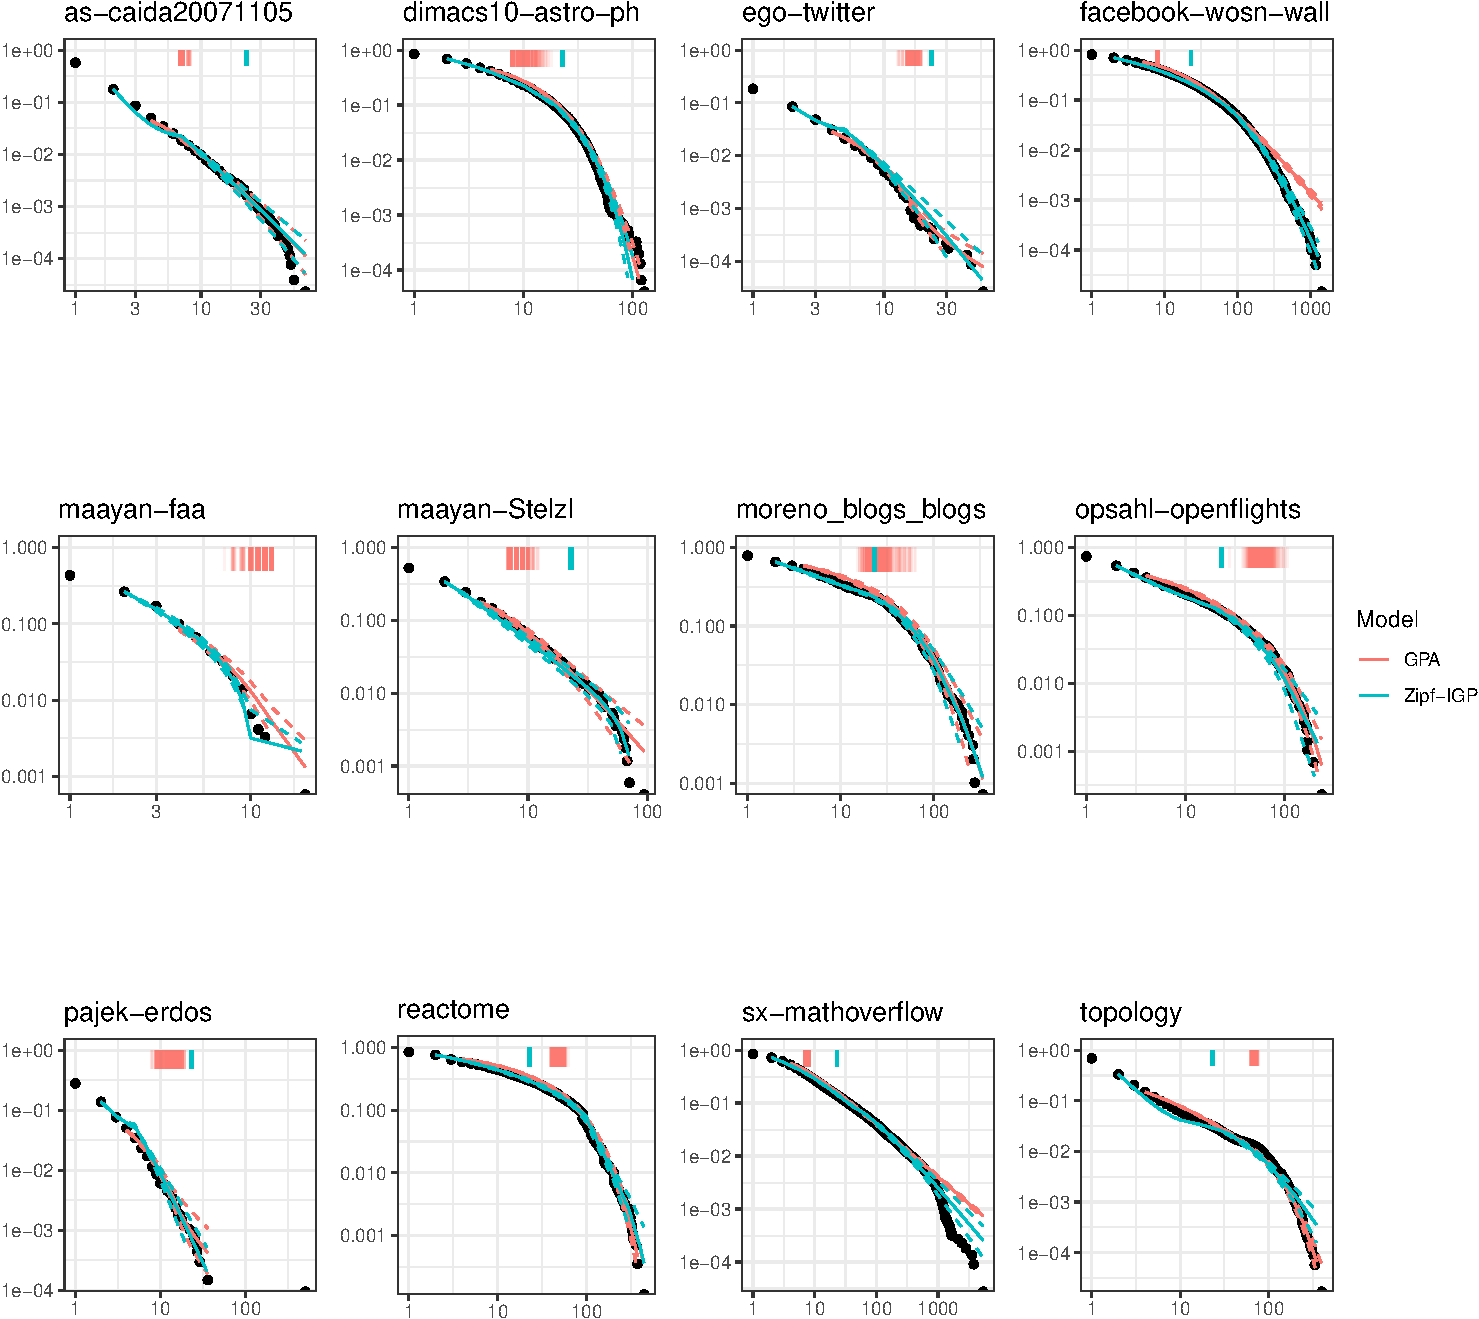
\includegraphics[width=1\linewidth,height=\textheight,keepaspectratio]{paper_files/figure-pdf/fig-real1-1.pdf}

}

\caption{\label{fig-real1}Empirical (black dots) and posterior medians
(solid red) of the fitted survival function for several real data sets
and their 95\% credible intervals (dotted red).}

\end{figure}%

Figure~\ref{fig-real1} displays the posterior estimates of the survival
function for various data sets, obtained from fitting the GPA model and
the Zipf-IGP mixture model from \citet{Lee24}. In most cases, the GPA
model gives a similar fit to the Zipf-IGP model but where the GPA model
fits well we gain additional information about the preference function,
assuming that the network evolved according the the GPA scheme.

\begin{figure}[H]

{\centering 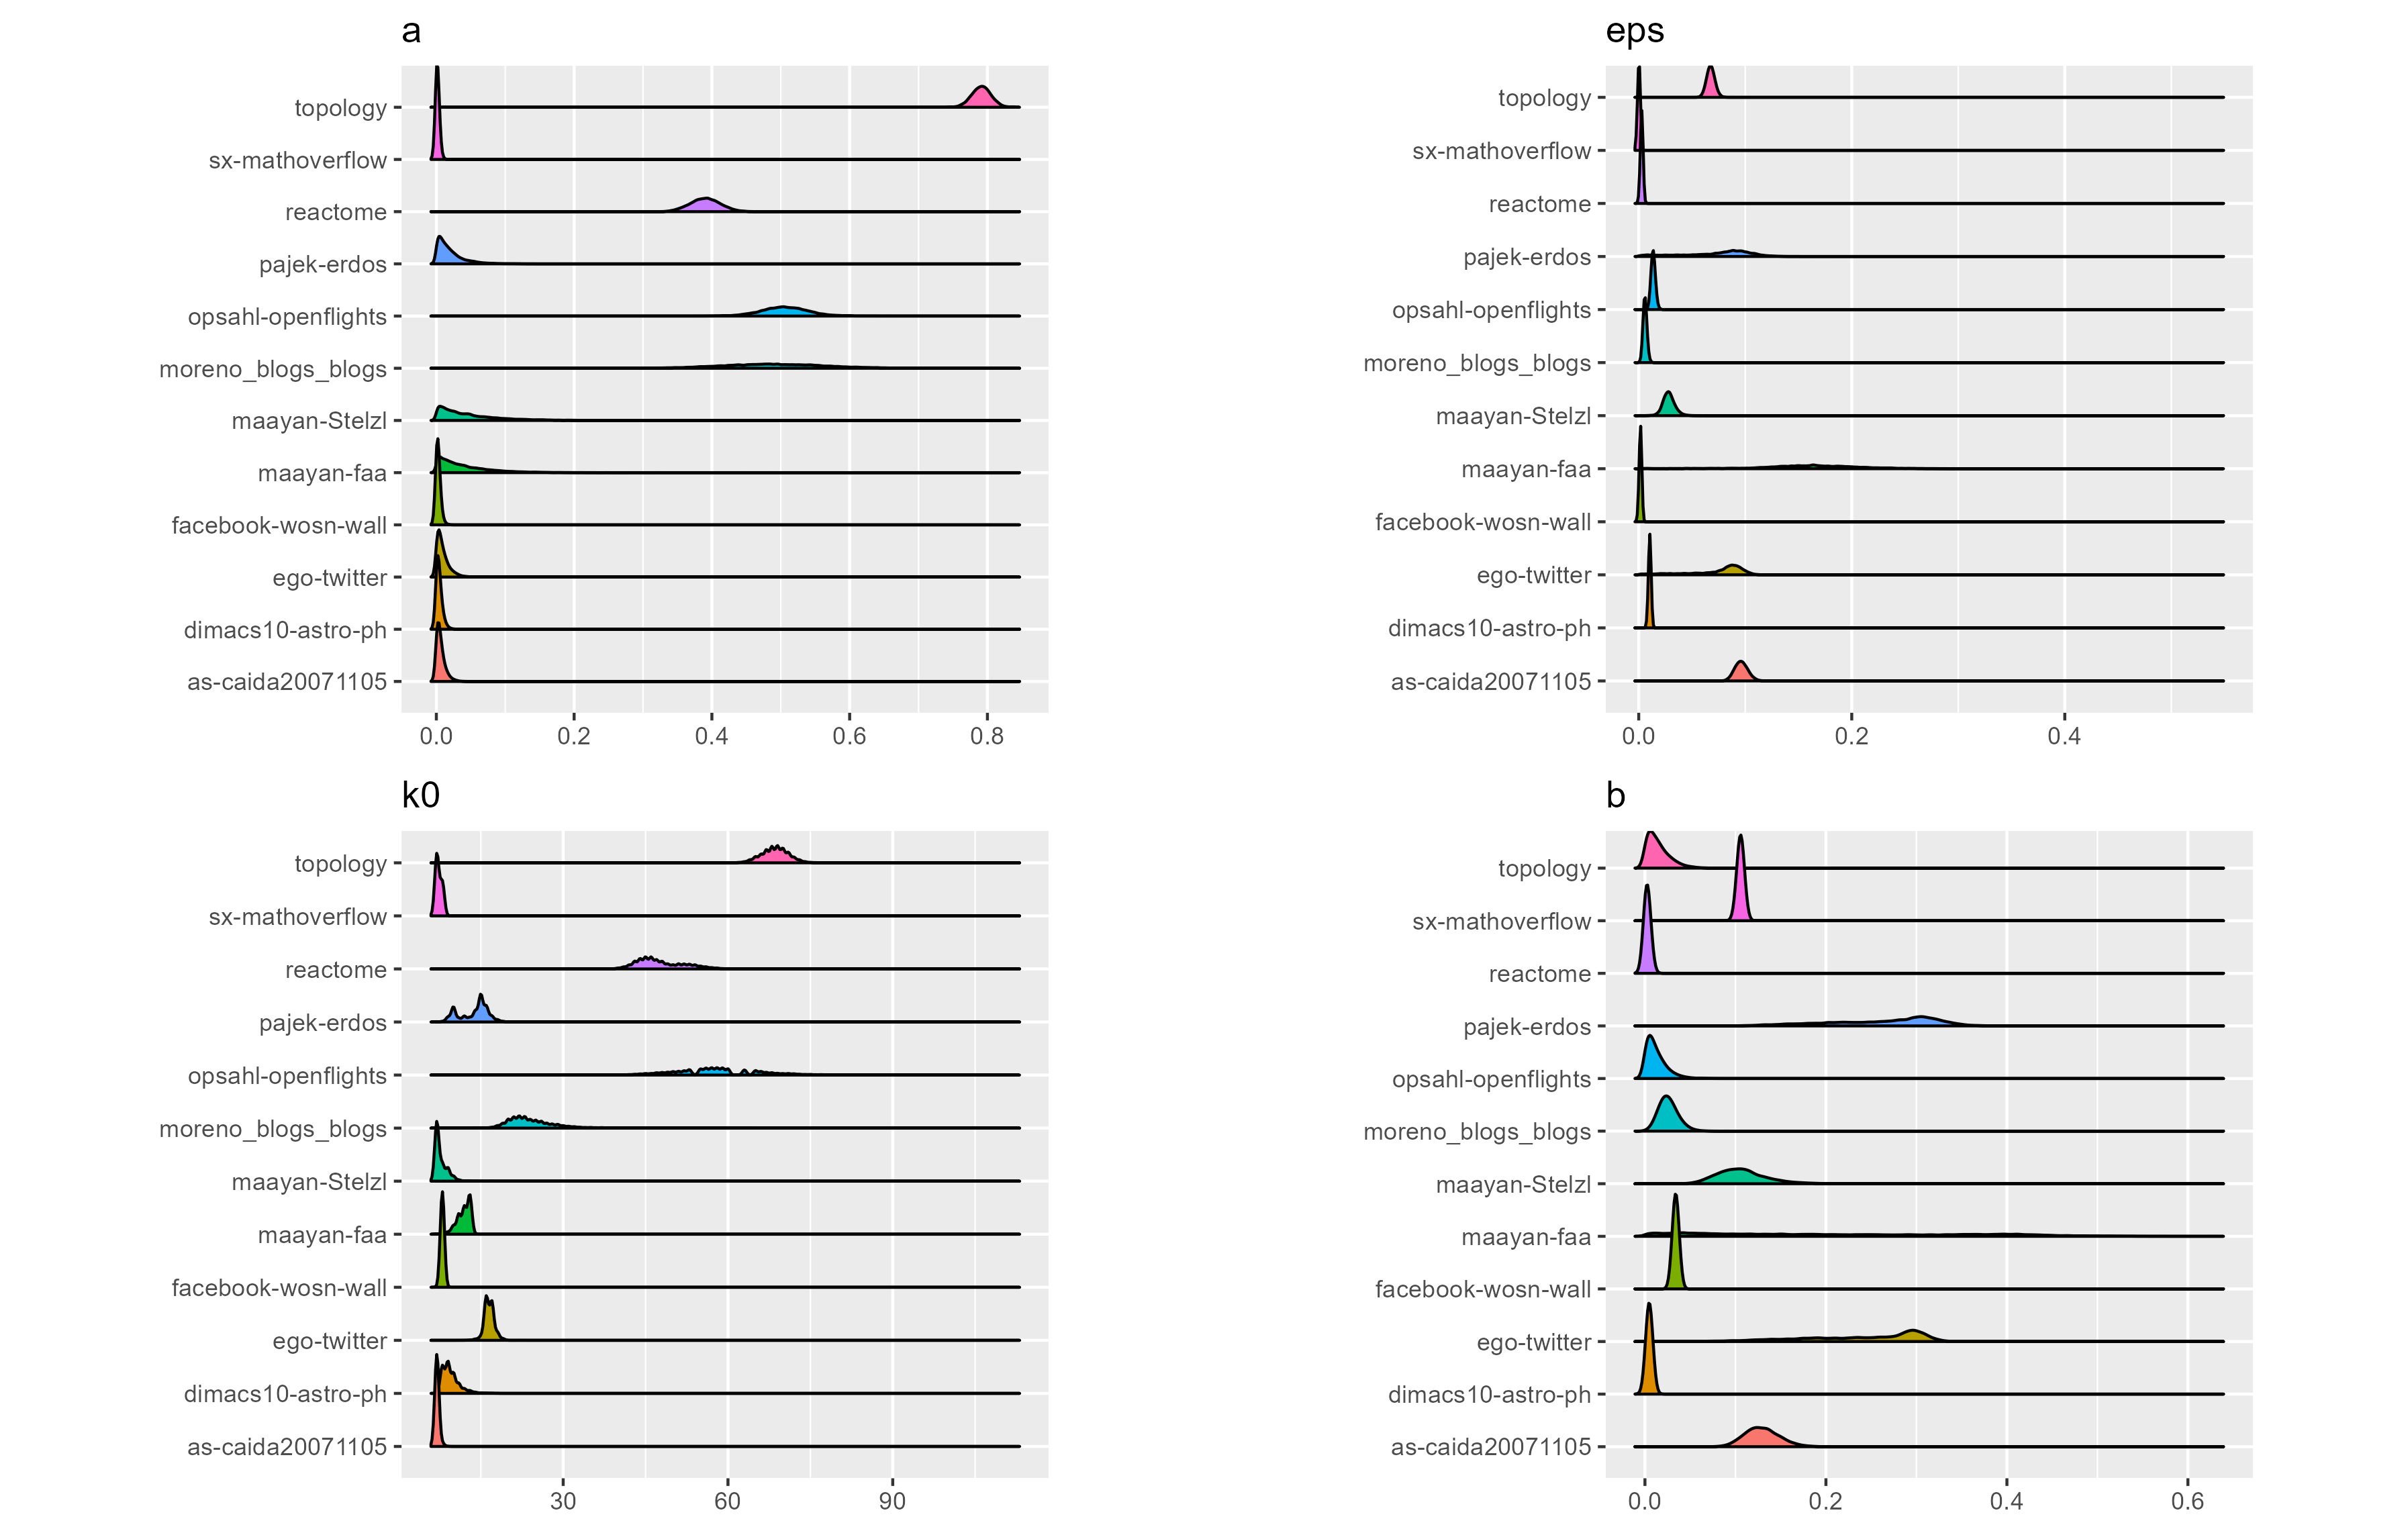
\includegraphics[width=0.8\linewidth,height=\textheight,keepaspectratio]{images/pars_plot.png}

}

\caption{Posterior densities of the parameters of the proposed model
fitted to real data.}

\end{figure}%

Figure~\ref{fig-shapes} shows the posterior of the shape parameter
\(\xi\) obtained from the Zipf-IGP model alongside the posterior of the
equivalent shape parameter \(\beta/\lambda^*\) obtained from fitting the
GPA model. Generally, the GPA model performs similarly to the Zipf-IGP
when estimating the tail behaviour of the degree distribution. In the
cases of substantial discrepancies, it is either because the GPA model
fits the tail better than the Zipf-IGP model does, or because of the
threshold being too low, forcing almost all of the data to be modelled
by the linear part of the GPA. This again shows the effects that small
degrees have on this model.

\begin{figure}

\centering{

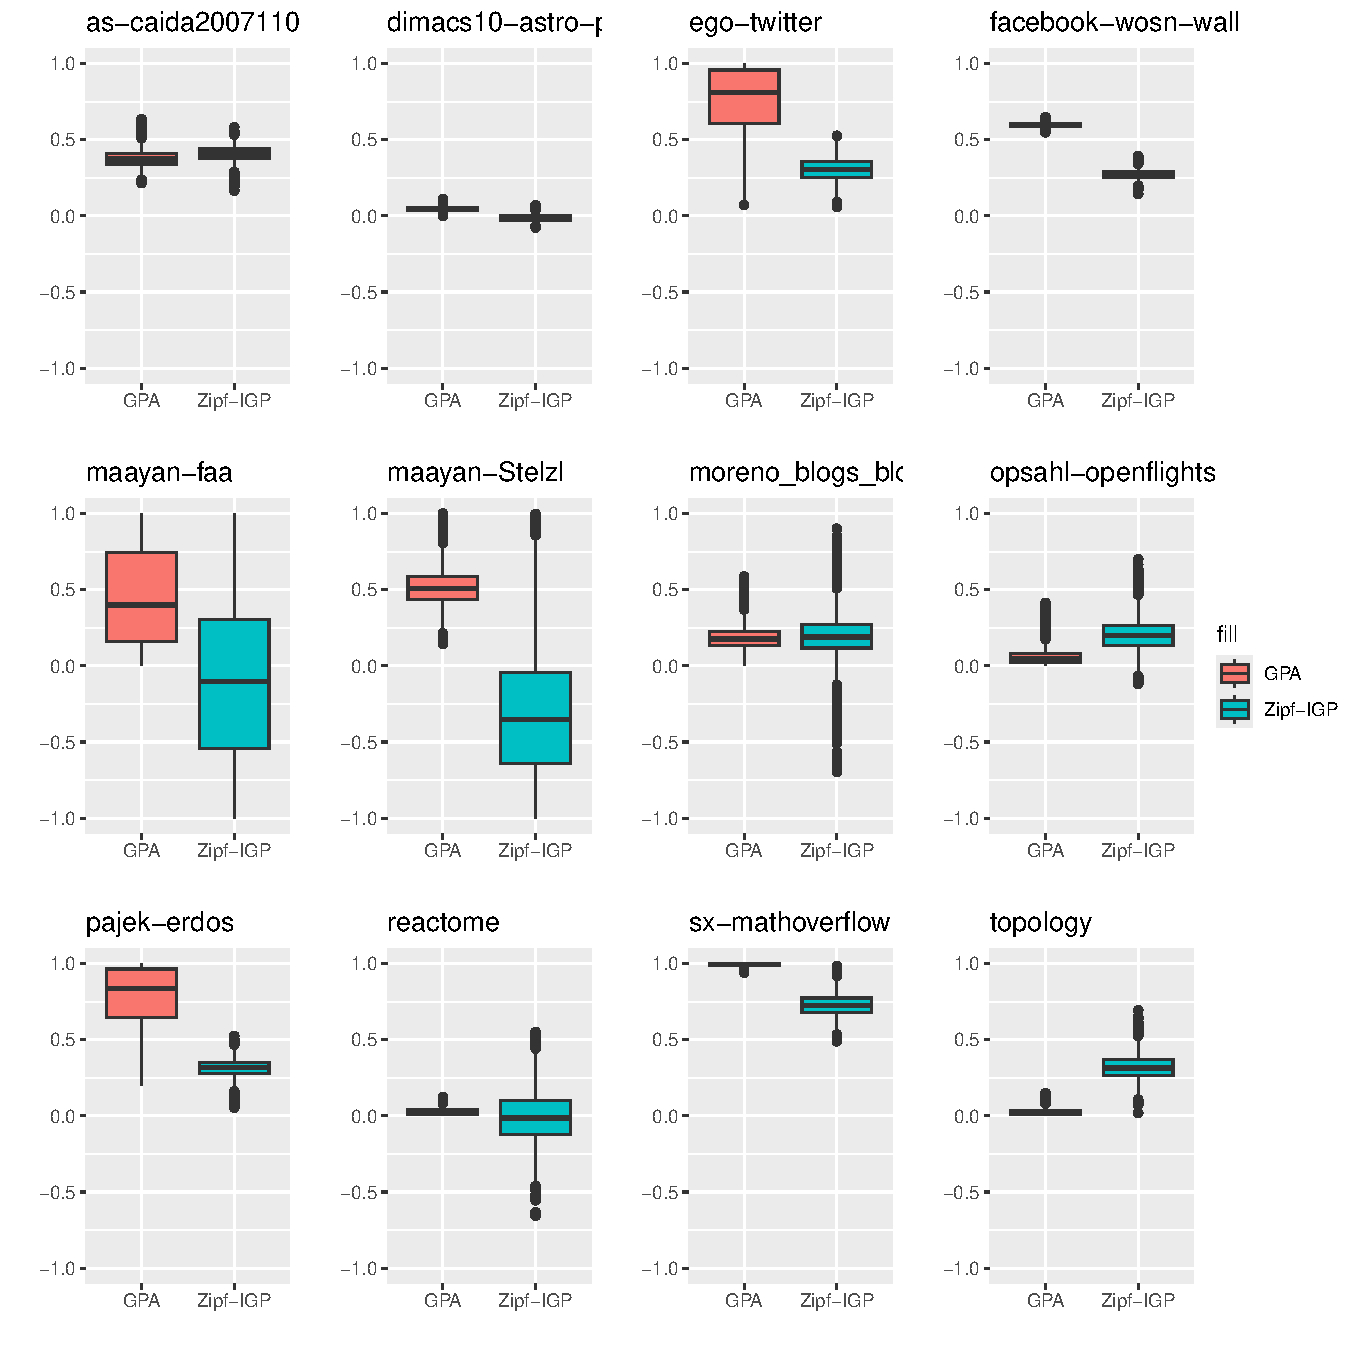
\includegraphics[width=1\linewidth,height=\textheight,keepaspectratio]{paper_files/figure-pdf/fig-shapes-1.pdf}

}

\caption{\label{fig-shapes}Posterior estimates of shape parameter of
Zipf-IGP distribution (right) and the analagous quantity obtained from
fitting the proposed model (left).}

\end{figure}%

Figure~\ref{fig-pa} shows the estimated preference function \(b(k)\)
alongside the 95\% credible interval on a log-log scale. Although the
credible interval becomes very large for the largest degrees, this is
expected as not all of these networks had data in that region, and for
those that do the credible interval is much narrower, as is the case for
\texttt{sx-mathoverflow}. Looking at the shape of the preference
function, there appears to be two distinct shapes of preference
function. The first appears mostly flat (similar to uniform attachment)
for the smallest degrees and then after a threshold PA kicks in, some
with this shape are \texttt{pajek-erdos} and \texttt{sx-mathoverflow}.
The second distinct shape appears to provide some clear PA behaviour
that then slows down after a certain point, and examples of this are
seen in the two infrastructure networks \texttt{opsahl-openflights} and
\texttt{topology}. This slowing down could be viewed as a kind of
diminishing returns on the degree of a vertex i.e.~as a vertex gets
larger gaining more connections has less of an effect than it did before
some threshold \(k_0\).

\begin{figure}

\centering{

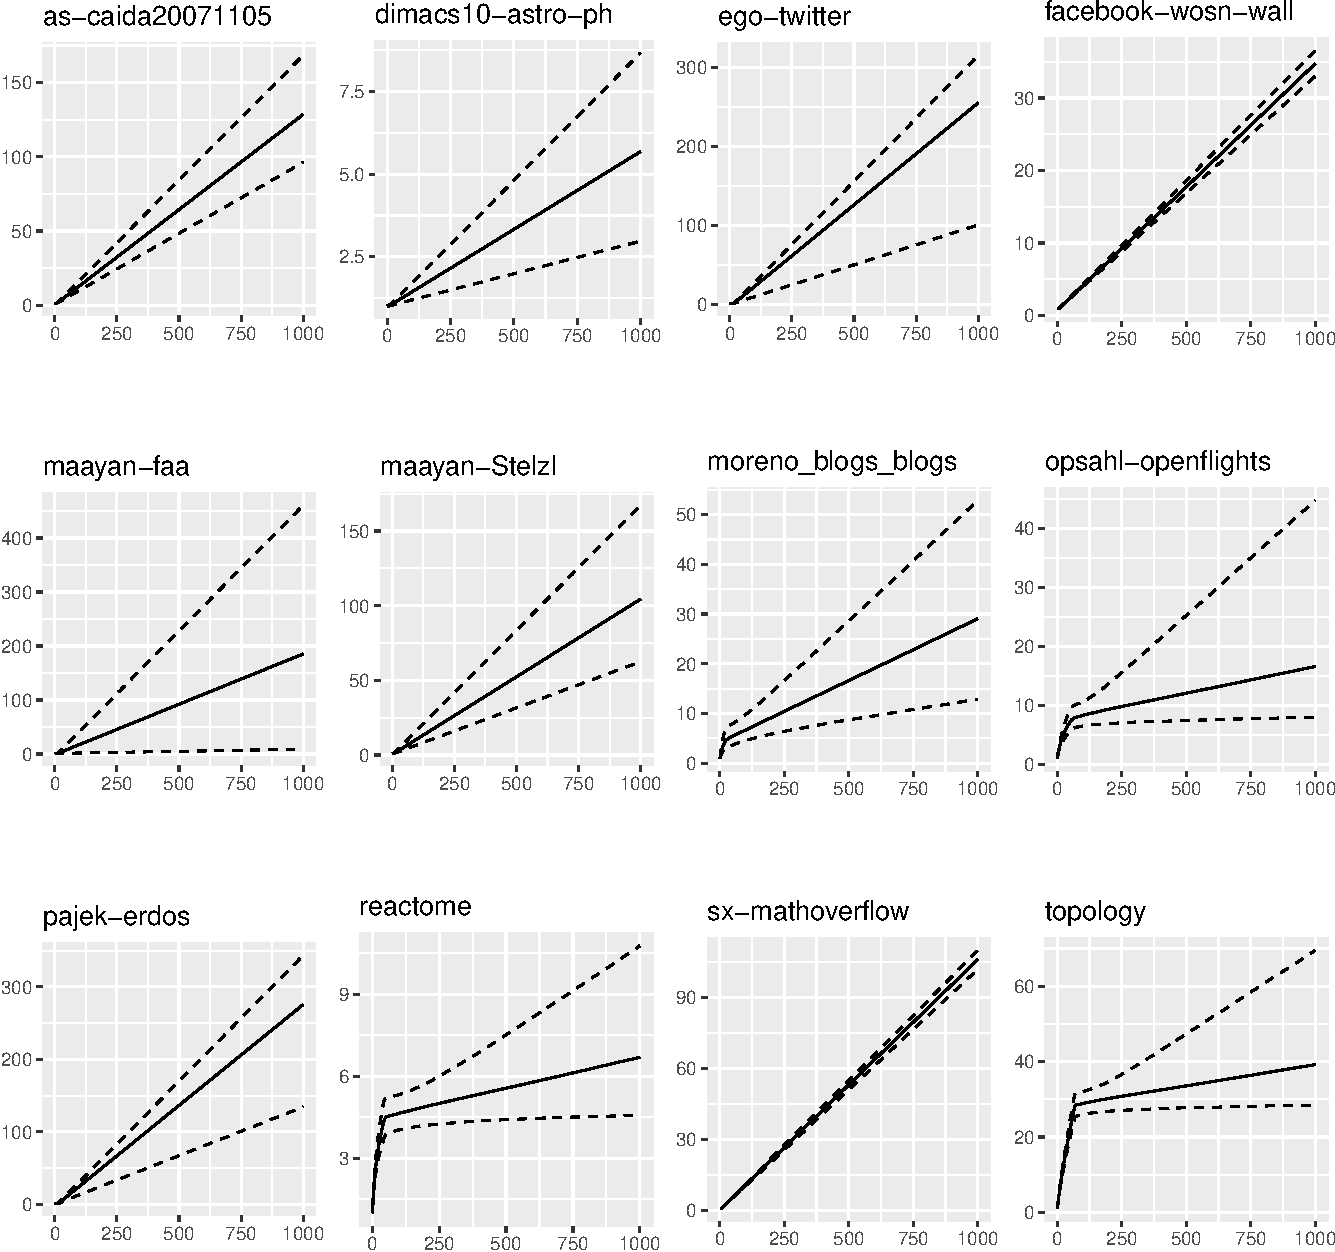
\includegraphics[width=0.8\linewidth,height=\textheight,keepaspectratio]{paper_files/figure-pdf/fig-pa-1.pdf}

}

\caption{\label{fig-pa}Posterior median for the preference function
(solid) with 95\% credible interval (dashed) on log-log scale.}

\end{figure}%

\newpage

\section{Conclusion and Discussion}\label{sec-conc}

In this paper we introduced a class of preference functions that, under
the GPA scheme, generate a network with a flexible yet regularly varying
degree distribution. From the simulation study we showed that the
parameters can be recovered from fitting the model to the degrees alone.
We also applied this method to the degree distributions of real
networks, estimating their model parameters assuming they evolved in the
same way. Not only did this yield fairly good fits for the degree
distribution, similar to that of the Zipf-IGP, it also came with the
added benefit of giving a posterior estimate for a preference function.

This paper contributes to the understanding of the relationship between
the mechanism underlying a networks growth and the resulting degree
distribution. As well as, demonstrating that under certain conditions
information about this mechanism can be garnered from the degrees alone.
Perhaps in future, something similar could be done by looking at another
statistic for the network (e.g.~the triangle distribution) and using it
in combination with the degrees to gain further insights into the growth
mechanism.

One limitation of this method is that the lowest degrees needed to be
truncated as they had a very large effect on the fit of the model, as a
result of using theory developed for trees and applying it to general
networks. Future work could apply theory developed for general networks
using a similar method to this, allowing us to compare the results here
something that is more accurate. This could include fixing the
out-degree of new nodes at a constant greater than one, or allowing the
out-degree of new nodes to vary.

Its worth noting the recent work by \citet{banerjee25}, that provides
results for more general networks beyond trees utilising the same
underlying branching process. They consider a model that grows in the
exact same way as the model that we have considered, but then they
collapse the nodes of the tree resulting in a more general network much
more like those in reality. However, there is no expression for the
probability mass function of the degrees and therefore no likelihood
that can be used for modeling in the same way that we have. In spite of
this, using Remark 2 from \citet{banerjee25} it can be shown that the
survival function of the limiting degree distribution (when using a
preference function of the form from Proposition~\ref{prp-omega2}) can
be bounded by two regularly varying functions showing that the degree
distribution is still heavy tailed, although not necessarily regularly
varying.

Obtaining an expression for the degree distributions of more general
cases of preferential attachment models are, for the moment, seemingly
inaccessible and provide a real barrier to using more realistic models
in a way similar to what we have in this paper, we leave these open
problems for future analysis.

\setcounter{section}{0}
\renewcommand{\thesection}{\Alph{section}}
\setcounter{table}{0}
\renewcommand{\thetable}{A\arabic{table}}
\setcounter{figure}{0}
\renewcommand{\thefigure}{A\arabic{figure}}

\newpage

\section{Supplementary Results}\label{sec-sup}

\begin{theorem}[Stolz-Cesàro Theorem
\citep{cesaro}]\protect\hypertarget{thm-stolz}{}\label{thm-stolz}

Let \((a_k)_{k\ge1}\) and \((b_k)_{k\ge1}\) be two sequence of real
numbers. Assume \((a_k)_{k\ge1}\) is a strictly monotone and divergent
sequence and the following limit exists:

\[
\lim_{k\rightarrow\infty}\frac{b_{k+1} - b_k}{a_{k+1} - a_k} = l.
\] Then,

\[
\lim_{k\rightarrow\infty}\frac{b_k}{a_k} = l.
\]

\end{theorem}

\section{Proofs and Derivations}\label{sec-proofs}

\subsection{\texorpdfstring{Proof of
Proposition~\ref{prp-omega}}{Proof of Proposition~}}\label{proof-of-prp-omega}

Taking the form of the GPA degree survival from
Equation~\ref{eq-surv-origin} : \[
\bar F(k) = \prod_{i=0}^k\frac{b(i)}{\lambda^*+b(i)}
\] and substituting into the formula for \(\Omega(F,n)\):

\begin{align*}
\Omega(F,k)&=\left(\log\frac{\prod_{i=0}^{k+1}\frac{b(i)}{\lambda+b(i)}}{\prod_{i=0}^{k+2}\frac{b(i)}{\lambda+b(i)}}\right)^{-1}-\left(\log\frac{\prod_{i=0}^{k}\frac{b(i)}{\lambda+b(i)}}{\prod_{i=0}^{k+1}\frac{b(i)}{\lambda+b(i)}}\right)^{-1}\\
&=\left(\log\frac{\lambda+b(k+2)}{b(k+2)}\right)^{-1}-\left(\log\frac{\lambda+b(k+1)}{b(k+1)}\right)^{-1}\\
&=\left(\log\left[1+\frac{\lambda}{b(k+2)}\right]\right)^{-1}-\left(\log\left[1+\frac{\lambda}{b(k+1)}\right]\right)^{-1}.
\end{align*}

Clearly if \(\lim_{k\rightarrow\infty}b(k)=c\) for some \(c>0\) then
\(\Omega(F,k)= 0 (= \lim_{k\rightarrow\infty}\frac{1}{\lambda^{*}} [b(k+2)-b(k+1)])\).
Now consider a non-constant \(b(k)\) and re-write \(\Omega(F,k)\) as:

\begin{align*}
\Omega(F,k) &= \left(\log\left[1+\frac{\lambda}{b(k+2)}\right]\right)^{-1}-\frac{b(k+2)}{\lambda}+\frac{b(k+2)}{\lambda}-\left(\log\left[1+\frac{\lambda}{b(k+1)}\right]\right)^{-1}\\&+\frac{b(k+1)}{\lambda}  -\frac{b(k+1)}{\lambda}\\
&=\left\{ \left(\log\left[1+\frac{\lambda}{b(k+2)}\right]\right)^{-1}-\frac{b(k+2)}{\lambda}\right\} - \left\{ \left(\log\left[1+\frac{\lambda}{b(k+1)}\right]\right)^{-1}-\frac{b(k+1)}{\lambda}\right\}\\&+\frac{b(k+2)}{\lambda}-\frac{b(k+1)}{\lambda}.
\end{align*}

Then if \(\lim_{k\rightarrow\infty}b(k)=\infty\) it follows that:

\begin{align*}
\lim_{k\rightarrow\infty}\Omega(F,k) &= \lim_{k\rightarrow\infty}\left\{ \left(\log\left[1+\frac{\lambda}{b(k+2)}\right]\right)^{-1}-\frac{b(k+2)}{\lambda}\right\} \\&- \lim_{k\rightarrow\infty}\left\{ \left(\log\left[1+\frac{\lambda}{b(k+1)}\right]\right)^{-1}-\frac{b(k+1)}{\lambda}\right\}\\
&\qquad+\lim_{k\rightarrow\infty}\left(\frac{b(k+2)}{\lambda}-\frac{b(k+1)}{\lambda}\right)\\
&=\frac{1}{2}-\frac{1}{2} + \lim_{k\rightarrow\infty}\left(\frac{b(k+2)}{\lambda}-\frac{b(k+1)}{\lambda}\right)\\
&=\frac{1}{\lambda}\lim_{k\rightarrow\infty}\left[b(k+2)-b(k+1)\right].\qquad \square
\end{align*}

\subsection{\texorpdfstring{Derivation of
Equation~\ref{eq-rho}}{Derivation of Equation~}}\label{derivation-of-eq-rho}

For a preference function of the form:

\[
b(k) = \begin{cases}
g(k),&k<k_0,\\
g(k_0) + \beta(k-k_0), &k\ge k_0,
\end{cases}
\] for \(\beta>0, k_0\in\mathbb N\) we have that

\begin{align*}
\hat\rho(\lambda) &= \sum_{n=0}^\infty\prod_{i=0}^{n-1}\frac{b(i)}{\lambda+b(i)}\\ &= \sum_{n=0}^{k_0}\prod_{i=0}^{n-1}\frac{g(i)}{\lambda+g(i)} + \sum_{n=k_0+1}^\infty\left(\prod_{i=0}^{k_0-1}\frac{g(i)}{\lambda+g(i)}\prod_{i=k_0}^{n-1}\frac{g(k_0) + \beta(i-k_0)}{\lambda +g(k_0) + \beta(i-k_0)}\right)\\
&=\sum_{n=0}^{k_0}\prod_{i=0}^{n-1}\frac{g(i)}{\lambda+g(i)} + \left(\prod_{i=0}^{k_0-1}\frac{g(i)}{\lambda+g(i)}\right)\sum_{n=k_0+1}^\infty\prod_{i=k_0}^{n-1}\frac{g(k_0) + \beta(i-k_0)}{\lambda +g(k_0) + \beta(i-k_0)}.
\end{align*}

Now using the fact that:

\[
\prod_{i=0}^n(x+yi) = x^{n+1}\frac{\Gamma\left(\frac{x}{y}+n+1\right)}{\Gamma\left(\frac{x}{y}\right)}
\] and reindexing the product in the second sum,

\begin{align*}
\hat\rho(\lambda) &= \sum_{n=0}^{k_0}\prod_{i=0}^{n-1}\frac{g(i)}{\lambda+g(i)} + \left(\prod_{i=0}^{k_0-1}\frac{g(i)}{\lambda+g(i)}\right)\sum_{n=k_0+1}^\infty\frac{\Gamma\left(\frac{g(k_0)}{\beta}+n-k_0\right)\Gamma\left(\frac{\lambda+g(k_0)}{\beta}\right)}{\Gamma\left(\frac{\lambda+g(k_0)}{\beta}+n-k_0\right)\Gamma\left(\frac{g(k_0)}{\beta}\right)}\\
&= \sum_{n=0}^{k_0}\prod_{i=0}^{n-1}\frac{g(i)}{\lambda+g(i)} + \frac{\Gamma\left(\frac{\lambda+g(k_0)}{\beta}\right)}{\Gamma\left(\frac{g(k_0)}{\beta}\right)}\left(\prod_{i=0}^{k_0-1}\frac{g(i)}{\lambda+g(i)}\right)\sum_{n=k_0+1}^\infty\frac{\Gamma\left(\frac{g(k_0)}{\beta}+n-k_0\right)}{\Gamma\left(\frac{\lambda+g(k_0)}{\beta}+n-k_0\right)}\\
&=\sum_{n=0}^{k_0}\prod_{i=0}^{n-1}\frac{g(i)}{\lambda+g(i)} + \frac{\Gamma\left(\frac{\lambda+g(k_0)}{\beta}\right)}{\Gamma\left(\frac{g(k_0)}{\beta}\right)}\left(\prod_{i=0}^{k_0-1}\frac{g(i)}{\lambda+g(i)}\right)\sum_{n=1}^\infty\frac{\Gamma\left(\frac{g(k_0)}{\beta}+n\right)}{\Gamma\left(\frac{\lambda+g(k_0)}{\beta}+n\right)}.
\end{align*}

In order to simplify the infinite sum, consider:

\begin{align*}
\sum_{n=0}^\infty\frac{\Gamma(n+x)}{\Gamma(n+x+y)} &=\frac{1}{\Gamma(y)}\sum_{n=0}^\infty \text{B}(n+x,y)\\
&=\frac{1}{\Gamma(y)}\sum_{n=0}^\infty\int_0^1t^{n+x-1}(1-t)^{y-1}at\\
&=\frac{1}{\Gamma(y)}\int_0^1 t^{x-1}(1-t)^{y-1}\sum_{n=0}^\infty t^n\,at\\
&=\frac{1}{\Gamma(y)}\int_0^1 t^{x-1}(1-t)^{y-1}\frac{1}{1-t}at\\
&=\frac{1}{\Gamma(y)}\int_0^1 t^{x-1}(1-t)^{y-2}at\\
&=\frac{1}{\Gamma(y)}\text{y}(x,y-1)\\
&= \frac{\Gamma(x)}{(y-1)\Gamma(x+y-1)}.
\end{align*}

This infinite sum does not converge when \(x\le1\) as each term is
\(O(n^{-x})\). We can now use this in \(\hat\rho(\lambda)\):

\begin{align*}
\hat\rho(\lambda) &= \sum_{n=0}^{k_0}\prod_{i=0}^{n-1}\frac{g(i)}{\lambda+g(i)} + \frac{\Gamma\left(\frac{\lambda+g(k_0)}{\beta}\right)}{\Gamma\left(\frac{g(k_0)}{\beta}\right)}\left(\prod_{i=0}^{k_0-1}\frac{g(i)}{\lambda+g(i)}\right)\left(\frac{\Gamma\left(\frac{g(k_0)}{\beta}\right)}{\left(\frac{\lambda}{\beta}-1\right)\Gamma\left(\frac{g(k_0)+\lambda}{\beta}-1\right)}-\frac{\Gamma\left(\frac{g(k_0)}{\beta}\right)}{\Gamma\left(\frac{g(k_0)+\lambda}{\beta}\right)}\right)\\
&=\sum_{n=0}^{k_0}\prod_{i=0}^{n-1}\frac{g(i)}{\lambda+g(i)} + \left(\prod_{i=0}^{k_0-1}\frac{g(i)}{\lambda+g(i)}\right)\left(\frac{\Gamma\left(\frac{g(k_0)+\lambda}{\beta}\right)}{\left(\frac{\lambda}{\beta}-1\right)\Gamma\left(\frac{g(k_0)+\lambda}{\beta}-1\right)}-1\right)\\
&=\sum_{n=0}^{k_0}\prod_{i=0}^{n-1}\frac{g(i)}{\lambda+g(i)} + \left(\prod_{i=0}^{k_0-1}\frac{g(i)}{\lambda+g(i)}\right)\left(\frac{\frac{g(k_0)+\lambda}{\beta}-1}{\frac{\lambda}{\beta}-1}-1\right)\\
&=\sum_{n=0}^{k_0}\prod_{i=0}^{n-1}\frac{g(i)}{\lambda+g(i)} + \left(\prod_{i=0}^{k_0-1}\frac{g(i)}{\lambda+g(i)}\right)\left(\frac{g(k_0)+\lambda-\beta}{\lambda-\beta}-1\right)\\&=\sum_{n=0}^{k_0}\prod_{i=0}^{n-1}\frac{g(i)}{\lambda+g(i)} + \frac{g(k_0)}{\lambda-\beta}\prod_{i=0}^{k_0-1}\frac{g(i)}{\lambda+g(i)}.\qquad \square
\end{align*}

\newpage

\section*{References}\label{references}
\addcontentsline{toc}{section}{References}

\renewcommand{\bibsection}{}
\bibliography{refs.bib}





\end{document}
